\section{Neutron Stars and Pulsars}

\subsection{A Prelude to Pulsars}

When stars with a mass of at least $8 \smass$ reach the end of their evolutionary stage they experience a depletion of nuclear fuel will and undergo a core collapse.  This results in the star exploding as a supernova. Depending on the mass of the host star the Supernova will form a black Hole or a neutron Star. Based on the electron degeneracy pressure limit \citep[pp. 434 -- 443]{chandrasekhar_introduction_2012} stars that fall in the range of 20 - 30 $\smass$ form neutron stars \citep{heger_how_2003}. \

Neutron stars are supported against further collapse by the presence of neutron degeneracy pressure which arises from the Pauli exclusion principle. Strong nuclear forces between the neutrons also provides additional support against gravitational collapse. With these three opposing forces a stable equilibrium is formed \citep{1983bhwd.book.....S}. \

In turn, this makes neutron stars exceptionally dense, they are the densest known objects in the universe that emit light. The average density of a neutron star is $10^{17} \text{kg/m}^3$ \citep{baym_neutron_1971} and their radii are comparable to the size of cities, with radii of 10--20 km. \

During collapse the conservation of magnetic flux plays a crucial role in the large strength magnetic fields that are observed in neutron stars along with contributions from the dynamo effect and frozen-in magnetic fields. The strength of a pulsar's magnetic field is on the order of $10^{12}$ - $10^{15}$ G \citep{michel_theory_1982}. \

Charged particles accelerate along the magnetic field lines in the magnetosphere of the neutron star. These particles emit electromagnetic radiation in a cone shape along the magnetic axis. If the magnetic axis is not aligned with the rotational axis of the neutron star, the radiation beam will sweep across the sky. This is known as a pulsar, a Galactic lighthouse.% analogus to cosmic lighthouses. 

\begin{figure}[t]
    \centering
    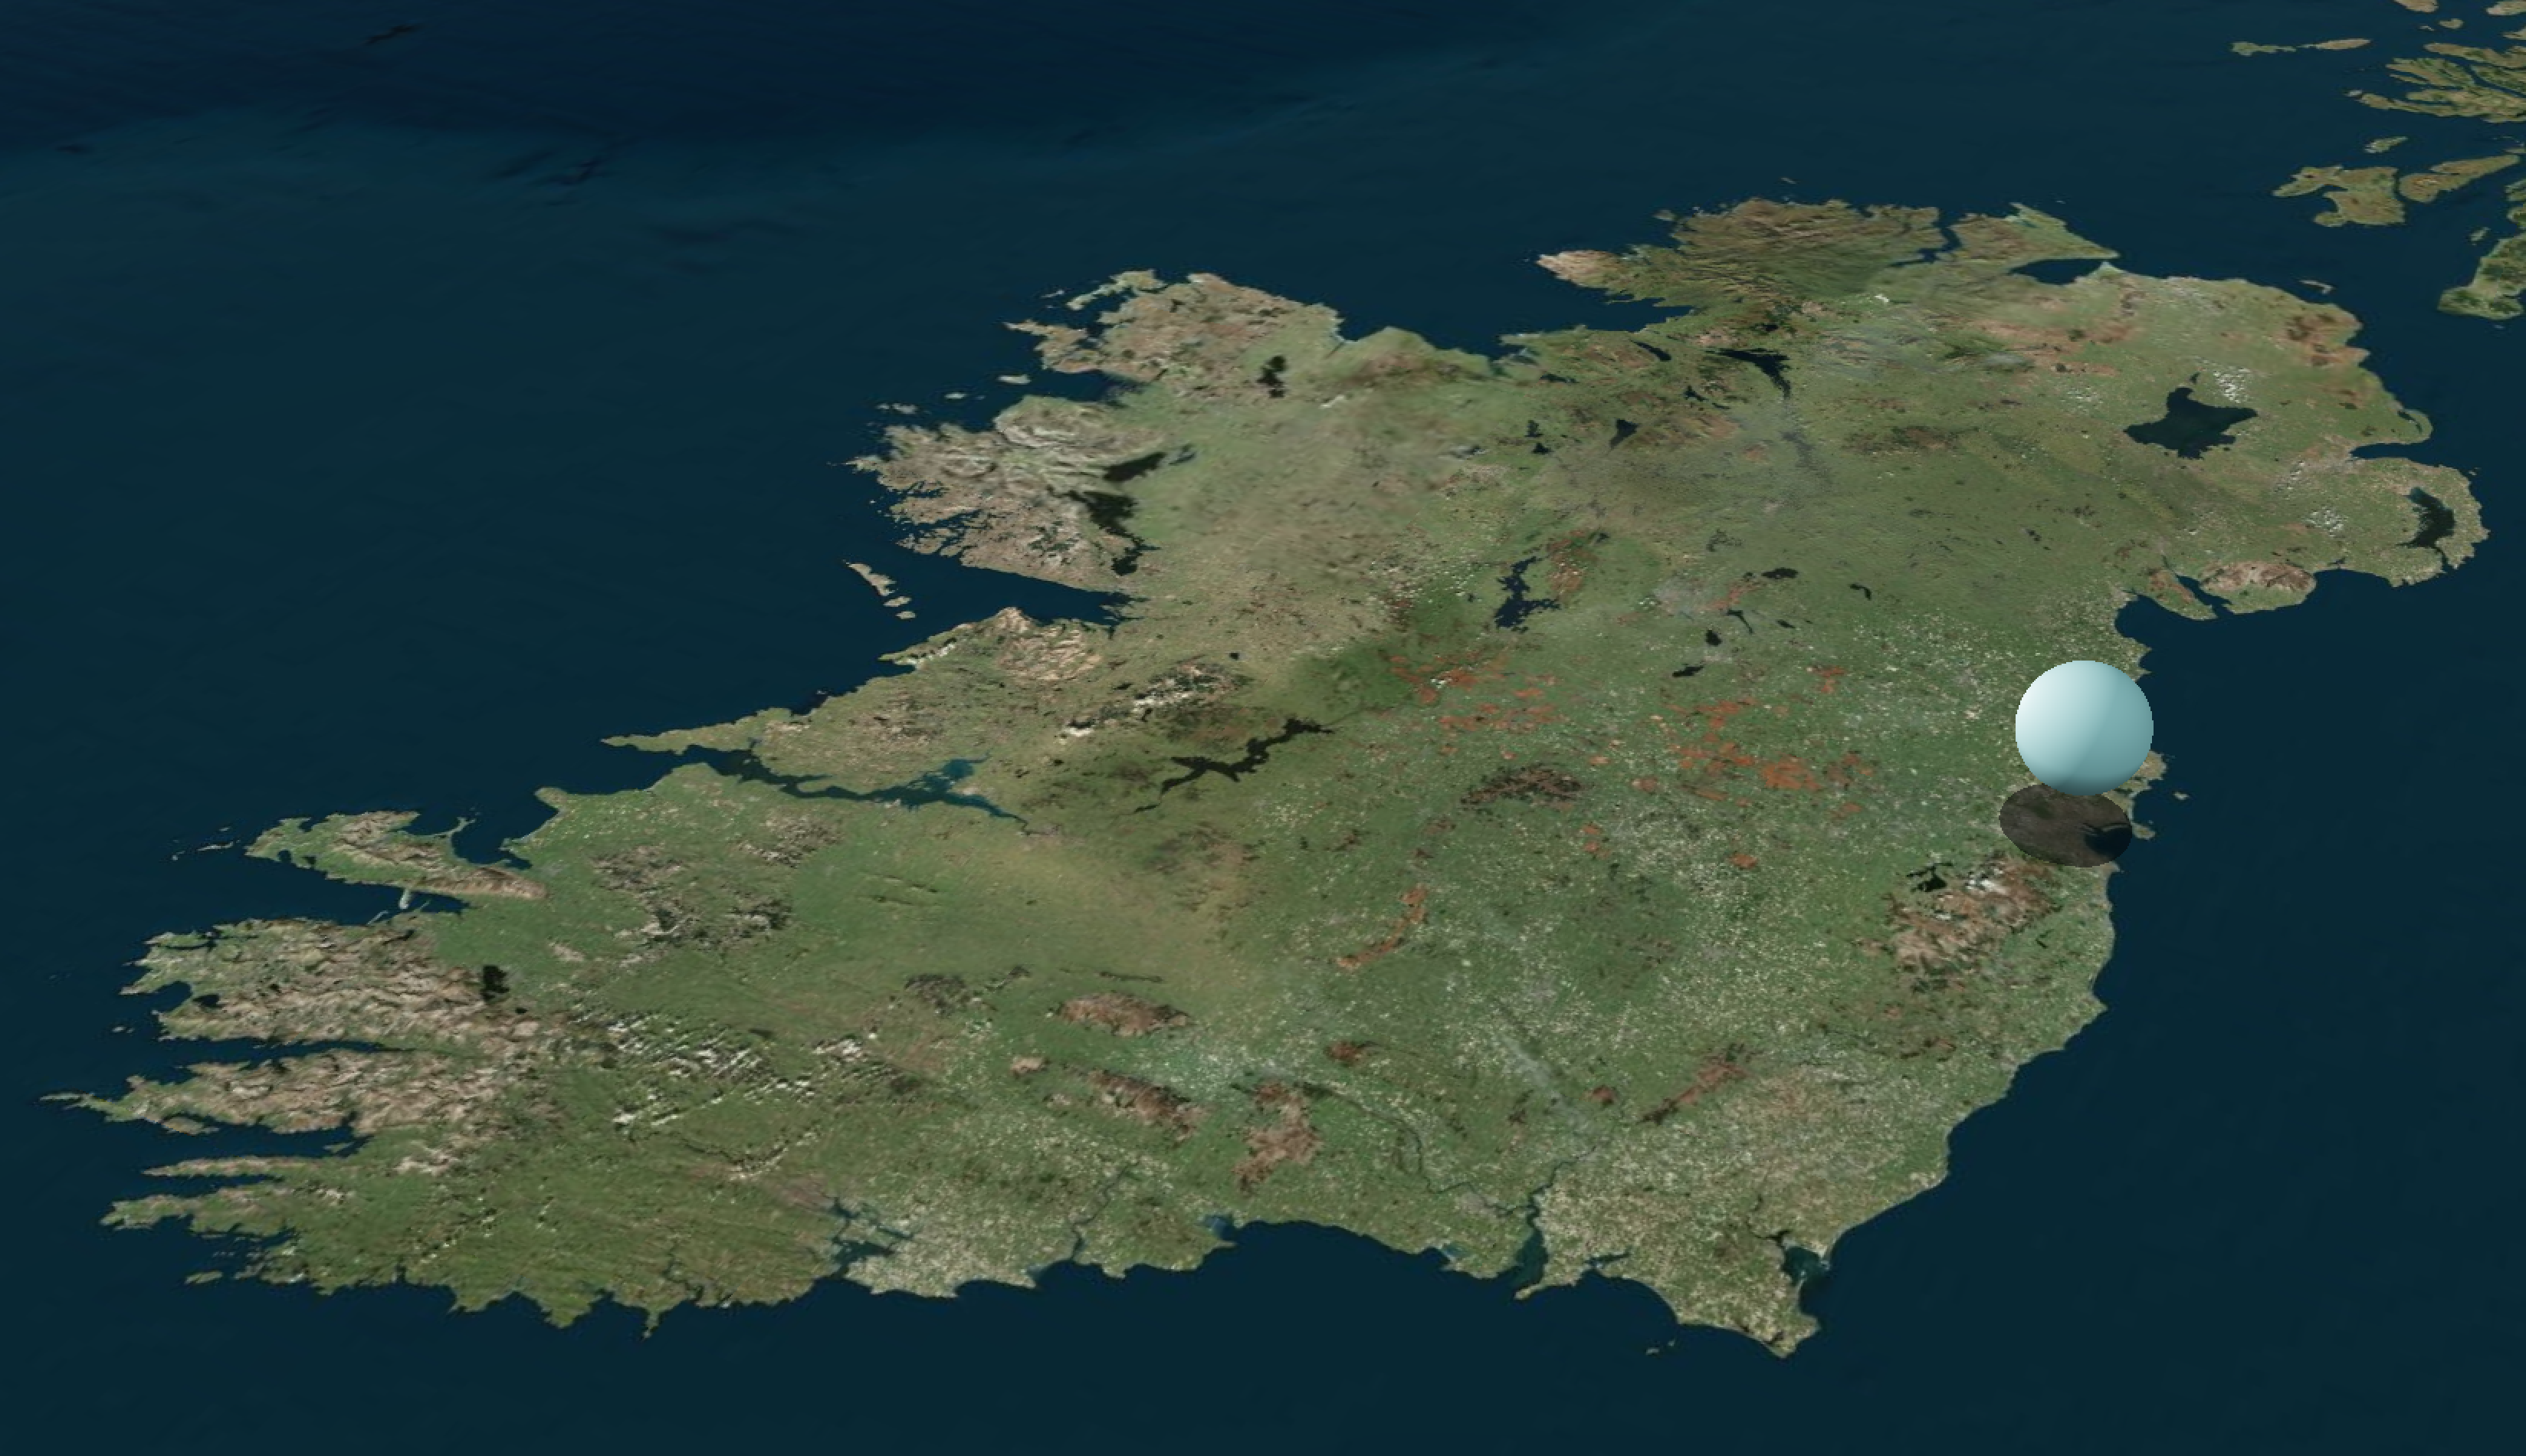
\includegraphics[width=0.8\linewidth]{chapter1/figures/ns-dublin.png}
    \caption{A canonical pulsar of $1.4 \smass$ positioned above House 1, Trinity College Dublin. Courtesy of Daniel Wysocki and HanGyeol Suh}
    \label{fig:placeholder}
\end{figure}


\subsection{The Population of Pulsars}

At the time of writing, there are currently more than 3380 known pulsars. Since their discovery by Jocelyn Bell Burnell \citep{hewish_observation_1968}, the population has grown immensely, but there remain many open questions about pulsar evolution and the subclasses that lie within the population as a whole. Similarly to how exoplanet populations are shown using the mass-radius diagram and stellar populations are shown using the Hertzsprung-Russell diagram, pulsar populations are shown using what is known as the $P-\dot P$ diagram.

$P$ represents the pulsar's rotational period and $\dot P$ its derivative. These are key ways that pulsars are classified and studied in the context of their evolution. An example of a $P-\dot P$ diagram is shown in \cref{fig:p-pdot}. Different values on the plot indicate roughly the pulsar's age and magnetic field strength. \Cref{fig:p-pdot} shows the vastly different values between pulsars in the millisecond range and pulsars in the second range.

Theoretically, it has been shown that pulsars can be related to a ``death" line in the $P-\dot P$ diagram. This is the line where pulsars are no longer able to emit radio waves due to the pulsar's magnetic field no longer being strong enough to accelerate particles along the magnetic field lines. However, it has been shown that pulsars do exist below this line. The area below this line is commonly referred to as the ``graveyard".

\begin{figure}
    \centering
    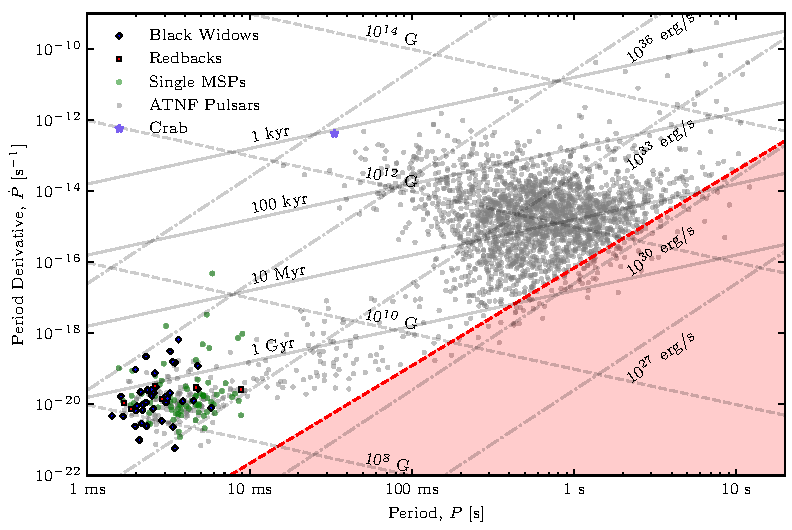
\includegraphics[width=0.8\textwidth]{chapter1/figures/PPdot-diagram.pdf}
    \caption{The $P-\dot P$ diagram showing the population of pulsars. The millisecond pulsar subclasses are colour coded. The red region represents the death line, where pulsars are theoretically no longer able to emit radio waves.}
    \label{fig:p-pdot}
\end{figure}

\subsection{The Properties of Pulsars}

The following section gives a brief non-exhaustive overview of some of the key properties of pulsars. 

\subsubsection{Neutron Star Radius \& Mass}

Understanding the mass of pulsars is important for understanding their evolution and equation of state. \cite{oppenheimer_massive_1939} derived a canonical mass limit of neutron stars to be 1.4 $\mathrm{M_{\odot}}$, but experimentally, this has been shown to be higher, with the largest mass of a pulsar observed to be $\sim 2.35 \mathrm{M_{\odot}}$ \citep{Romani_2022}. The mass-radius relationship of a pulsar is defined by an equation of state and a maximum mass limit. Redshifts and gravitational effects observed in pulsars exhibit the observed temperature and flux to be smaller than the actual value. The observed radius $R_\text{obs}$ can be described as follows \citep[p. 56][]{pulsar_handbook}:

\begin{equation}
    R_\text{obs} = \frac{R}{\sqrt{1 - \frac{2GM}{Rc^2}}} = \frac{R}{ \sqrt{1 - \dfrac{R_s}{R}}}
\end{equation}

where $R$ is the pulsar's radius and $M$ is the gravitational mass, $G$ is the gravitational constant, $c$ is the speed of light and $R_s$ is the Schwarzschild radius. \
The lower limit of the neutron star radius is described by \cite[p. 58][]{pulsar_handbook}: 

\begin{equation}
    R_\text{min} \simeq 1.5 \ R_s = \frac{3GM}{c^2} = 6.2 \ \text{km.} \left( \frac{M}{1.4 \smass} \right)
\end{equation}

Opposite to this the upper limit of the radius is obtained by requiring that there is stability against breaking up due to centrifugal forces. This gives \cref{eq:radius-max} following as described in \cite[p.~58]{pulsar_handbook}. 

\begin{equation}
    R_\text{max} \simeq \left(\frac{GMP^2}{4 \pi^2}\right)^{1/3} = 16.8 \ \text{km} \left( \frac{M}{1.4 \smass} \right)^{1/3} \left( \frac{P}{\text{ms}} \right)^{2/3}
    \label{eq:radius-max}
\end{equation}

Most pulsars are theoretically thought to have radii in the range of 10–15 km \citep{lattimer_neutron_2001}, giving them the unique position of `almost' black holes. 

\subsubsection{Spin Evolution}
One of the unique characteristics of pulsars is the spinning that they exhibit. Understanding the spin evolution gives insight into many parameters of the pulsars, most notably the stage of their evolution. Pulsars begin their life in the upper end of the $P-\dot P$ diagram and slowly move down and to the right as they age due to a loss in rotational energy, commonly referred to as spin-down luminosity. The spin-down ($\dot E$) is described as follows \citep[p.~59]{pulsar_handbook}:

\begin{equation}
\dot E = - \frac{dE_{\text{rot}}}{dt} = 4\pi^2 I \dot P P^{-3}
\label{eq:spin-down-energy}
\end{equation}

Where $I$ is the moment of inertia. It is important to note that the energy loss that is converted into radio emission is almost negligible in comparison to the total energy loss from spin down. 

% \subsubsection{Radio Emission Beam}

% Pulse width

% \begin{equation}
%     \cos \rho = \cos \alpha \cos (\alpha + \beta) + \sin \alpha \sin (\alpha + \beta) \cos \left( \frac{W}{2} \right)
% \end{equation}

\subsubsection{Braking Index}

Pulsars have strong magnetic dipoles. According to classical mechanics, a rotating magnetic dipole that exhibits a moment, $|m|$, emits an electromagnetic wave at the pulsar's rotation frequency \citep[p.~60]{pulsar_handbook}. The dipole's radiation power is characterized by:

\begin{equation}
    \dot E_{\text{dipole}} = \frac{2}{3c^3} |m|^2 \omega^4 \sin^2 \alpha
\end{equation}

Where $\alpha$ is the angle between the magnetic axis and the rotation axis. Equating the above equation to the loss of rotational energy described in \cref{eq:spin-down-energy} gives the following for the expected evolution of the period:

\begin{equation}
    \dot \Omega = - \frac{2}{3Ic^3} |m|^2 \Omega^3 \sin^2 \alpha
\end{equation}

This is more commonly written as a power law, 

\begin{equation}
    \dot \nu = -K \nu^n 
    \label{eq:spin-down-power-law}
\end{equation}

\Cref{eq:spin-down-power-law} in terms of the period is $\dot P = K P^{2-n}$. Since this is a first-order differential equation, the solution can be integrated and given a constant, $K$, which provides an expression of age:

\begin{equation}
    T = \frac{P}{(n-1)\dot P} \left\{ 1 - \left( \frac{P_0}{P} \right)^{n - 1} \right\} 
    \label{eq:age-full}
\end{equation}

Here $P_0$ is the initial period of the pulsar. Commonly an assumption is made that the current period is much greater than the initial period $(P_0 \ll P)$. If it is also assumed that the pulsar is spinning down to due dipole magnetic radiation ($n=3$), \cref{eq:age-full} can be simplified into a characteristic age. 

\begin{equation}
    \tau_c \cong 15.8~\text{Myr} \left( \frac{P}{s} \right) \left( \frac{\dot P}{10^{-15}} \right)^{-1}
\end{equation}

The above estimation for a pulsars age is known to be inconsistent with theory to varying degrees. In cases where Supernovae has been observed and has produced a pulsar the age is known to a much higher degree of accuracy. The Crab pulsar is one such example with an observed Supernova event in 1054 AD by Chinese astronomers \citep{kaspi_chandra_2001}. %Supernoave remnants are also used to estimate the age of pulsars. 

\subsubsection{Dispersion Measure} \label{sec:DispersionMeasure}

The interstellar medium (ISM) is a complex mixture of gas, dust and magnetic fields that fills the space between stars in a galaxy. Given that the ISM is a cold and ionised plasma any electromagnetic radiation will undergo a frequency-dependant index of refraction as they propagate. The following equation describes the refractive index of the ISM neglecting Galactic magnetic field \citep[p.~85]{pulsar_handbook},

\begin{equation}
    \mu = \sqrt{1 - \left( \frac{f_p}{f} \right)^2}
    \label{eq: ism-refractive-index}
\end{equation}

Where $f_p$ is the plasma frequency, $8.5 ~\text{kHz} \left(n_e/\text{cm}^{-3} \right)^{1/2}$ and $f$ is the frequency of the observed radiation. \\ If the refractive index of the ISM $\mu < 1$ then it can be assumed that the group velocity of the radiation is $v_g = c\mu$ which is sub light speed. The path of radiation from a pulsar to the observer will be delayed in time with respect to an infinite frequency by an amount:

\begin{equation}
    t = \left( \int^d_0 \frac{dl}{v_g} \right) - \frac{d}{c}
\end{equation}

If is assumed to be $f_p \ll f$, $\mu$ can be approximated.

\begin{equation}
    t = \frac{1}{c} \int^d_0 \left(1 + \frac{f_p^2}{2f^2} \right) dl - \frac{d}{c}  = \frac{e^2}{2 \pi m_e c} \dfrac{\int^d_0 n_e ~dl}{f^2} \equiv \mathcal{D} \cdot \dfrac{\text{DM}}{f^2}
\end{equation}

Where $\mathcal{D}$ is the dispersion constant and $\text{DM}$ is the dispersion measure. Each are commonly expressed as follows, $\mathcal{D}= 4.15 \times 10^3 ~\text{MHz}^2 ~\text{pc}^{-1} ~ \text{cm}^3 ~\text{s}$ and $\text{DM} = \int^d_0 n_e ~dl ~\text{cm}^{-3} ~\text{pc}$. This definition was adapted from \citet[p.~86]{pulsar_handbook} and \cite{taylor_recent_1977}.